\documentclass[acmsmall, nonacm]{acmart}

\usepackage[english]{babel}
\usepackage{array}
\usepackage{fancyvrb}
\usepackage{hyperref}
\usepackage{relsize}
\usepackage{textcomp}
\usepackage{xcolor}
\usepackage{xspace}
\usepackage{booktabs}
\usepackage{listings}
\usepackage{smartdiagram}
\usepackage{scalefnt}
\usepackage[nolist]{acronym}

\usetikzlibrary{shapes}
\usetikzlibrary{intersections}
\usetikzlibrary{calc}
\usetikzlibrary{optics}
\usetikzlibrary{arrows}
\usetikzlibrary{positioning}
\usetikzlibrary{decorations}
\usetikzlibrary{angles}
\usetikzlibrary{quotes}
\usetikzlibrary{arrows.meta,shapes.geometric,decorations.pathreplacing}

\definecolor{backcolour}{rgb}{0.95,0.95,0.92}

\lstdefinestyle{codestyle}{
    backgroundcolor=\color{backcolour},
    basicstyle=\ttfamily\footnotesize,
    breakatwhitespace=false,
    breaklines=true,
    captionpos=b,
    keepspaces=true,
    numbersep=5pt,
    showspaces=false,
    showstringspaces=false,
    showtabs=false,
    tabsize=2
}

\addto\extrasenglish{
    \def\sectionautorefname{Section}
    \def\subsectionautorefname{\sectionautorefname}
    \def\subsubsectionautorefname{\sectionautorefname}
    \def\paragraphautorefname{Paragraph}
    \def\subparagraphautorefname{\paragraphautorefname}
}

\lstset{style=codestyle}

\usepackage{siunitx}
\sisetup{per-mode=symbol}
\sisetup{sticky-per=true}				% every unit behind "per" is reciprocal

\newcolumntype{L}[1]{>{\raggedright\let\newline\\\arraybackslash\hspace{0pt}}m{#1}}
\newcolumntype{C}[1]{>{\centering\let\newline\\\arraybackslash\hspace{0pt}}m{#1}}

\definecolor{olivegreen}{rgb}{0.0, 0.6, 0.0}
\definecolor{darkred}{rgb}{0.7, 0.0, 0.0}
\definecolor{orangeyellow}{rgb}{0.9, 0.7, 0.2}
\newcommand{\red}[1]{\textcolor{darkred}{#1}}
\newcommand{\orange}[1]{\textcolor{orangeyellow}{#1}}
\newcommand{\green}[1]{\textcolor{olivegreen}{#1}}
\newcommand{\unitof}[1]{\ensuremath{\left[#1\right]}}

\newcommand{\sansserifformat}[1]{\fontfamily{cmss}{ #1}}%

\newcommand{\gh}{GitHub\xspace}
\newcommand{\gl}{GitLab\xspace}
\newcommand{\git}{Git\xspace}
\newcommand{\docx}{\textit{.docx}\xspace}
\newcommand{\wftw}{Word for the Web\xspace}
\newcommand{\magit}{markup\,+\,\git}

% Typeset from the C++ standard
\newcommand{\Rplus}{\protect\hspace{-.1em}\protect\raisebox{.35ex}{\smaller{\smaller\textbf{+}}}}
\newcommand{\Cpp}{\mbox{C\Rplus\Rplus}\xspace}

%
%% \BibTeX command to typeset BibTeX logo in the docs
\AtBeginDocument{%
\providecommand\BibTeX{{%
\normalfont B\kern-0.5em{\scshape i\kern-0.25em b}\kern-0.8em\TeX}}}

%% Rights management information.  This information is sent to you
%% when you complete the rights form.  These commands have SAMPLE
%% values in them; it is your responsibility as an author to replace
%% the commands and values with those provided to you when you
%% complete the rights form.
\copyrightyear{}
\acmYear{}
\setcopyright{none}

%% These commands are for a PROCEEDINGS abstract or paper.
% \acmConference[HCI]{Conference}{Date}{Location}
\acmBooktitle{}
\acmPrice{}
\acmISBN{}
\acmDOI{}

%%
%% Submission ID.
%% Use this when submitting an article to a sponsored event. You'll
%% receive a unique submission ID from the organizers
%% of the event, and this ID should be used as the parameter to this command.
\acmSubmissionID{}

%%
%% The majority of ACM publications use numbered citations and
%% references.  The command \citestyle{authoryear} switches to the
%% "author year" style.
%%
%% If you are preparing content for an event
%% sponsored by ACM SIGGRAPH, you must use the "author year" style of
%% citations and references.
%% Uncommenting
%% the next command will enable that style.
%%\citestyle{acmauthoryear}

%%
%% end of the preamble, start of the body of the document source.
\begin{document}

%%
%% The "title" command has an optional parameter,
%% allowing the author to define a "short title" to be used in page headers.
\title{Large-Scale Collaborative Writing: Technical Challenges and Recommendations}

%%
%% The "author" command and its associated commands are used to define
%% the authors and their affiliations.
%% Of note is the shared affiliation of the first two authors, and the
%% "authornote" and "authornotemark" commands
%% used to denote shared contribution to the research.
%\author{************** Paper ID 2303 **************}

\author{Markus Hofbauer}
\authornote{Both authors contributed equally to this research.}
\email{markus.hofbauer@tum.de}
\orcid{0000-0002-8167-5485}
\affiliation{%
    \institution{Technical University of Munich}
    \department[2]{School of Computation, Information and Technology}
    \department[1]{Department of Computer Engineering}
    \department[0]{Chair of Media Technology}
    \department[0]{Munich Institute of Robotics and Machine Intelligence (MIRMI)}
    \city{Munich}
    \state{Bavaria}
    \country{Germany}
    \and
    \institution{Luminar Technologies, Inc.}
    \city{Munich}
    \state{Bavaria}
    \country{Germany}
}

\author{Christoph Bachhuber}
\authornotemark[1]
\email{christoph.bachhuber@luminartech.com}
\orcid{0000-0002-9808-0162}
\affiliation{%
    \institution{Luminar Technologies, Inc.}
    \city{Munich}
    \state{Bavaria}
    \country{Germany}
}

\author{Christopher Kuhn}
\email{christopher.kuhn@tum.de}
\orcid{0000-0002-0107-0516}
\affiliation{%
    \institution{Technical University of Munich}
    \department[2]{School of Computation, Information and Technology}
    \department[1]{Department of Computer Engineering}
    \department[0]{Chair of Media Technology}
    \department[0]{Munich Institute of Robotics and Machine Intelligence (MIRMI)}
    \city{Munich}
    \state{Bavaria}
    \country{Germany}
}

\author{Sebastian Schwarz}
\email{sebastian.schwarz@nokia.com}
\affiliation{%
    \institution{Nokia Technologies}
    \city{Munich}
    \state{Bavaria}
    \country{Germany}
}

\author{Bart Kroon}
\email{bart.kroon@philips.com}
\affiliation{%
    \institution{Philips Research Eindhoven}
    \city{Munich}
    \state{Bavaria}
    \country{Germany}
}

\author{Eckehard Steinbach}
\email{eckehard.steinbach@tum.de}
\orcid{0000-0001-8853-2703}
\affiliation{%
    \institution{Technical University of Munich}
    \department[2]{School of Computation, Information and Technology}
    \department[1]{Department of Computer Engineering}
    \department[0]{Chair of Media Technology}
    \department[0]{Munich Institute of Robotics and Machine Intelligence (MIRMI)}
    \city{Munich}
    \state{Bavaria}
    \country{Germany}
}

\begin{acronym}
    \acro{LDA}{\emph{Latent Dirichlet Allocation}}
    \acro{CMT}{\emph{Conference Management Toolkit}}
    \acro{TPMS}{\emph{The Toronto Paper Matching System}}
    \acro{MCMF}{\emph{MinCost-MaxFlow}}
\end{acronym}

%%
%% By default, the full list of authors will be used in the page
%% headers. Often, this list is too long, and will overlap
%% other information printed in the page headers. This command allows
%% the author to define a more concise list
%% of authors' names for this purpose.
% \renewcommand{\shortauthors}{Hofbauer, Bachhuber, Kuhn, Schwarz, Kroon, and Steinbach}

%%
%% The abstract is a short summary of the work to be presented in the
%% article.
\begin{abstract}
    Collaborative writing is essential for teams that create documents together.
    Creating documents in large-scale collaborations is a challenging task that requires an efficient workflow.
    The design of such a workflow has received comparatively little attention.
    Conventional solutions such as working on a single Microsoft Word document or a shared online document are still widely used.
    In this paper, we propose a new workflow consisting of a combination of the lightweight markup language AsciiDoc together with the state-of-the-art \acl{VCS} \git.
    The proposed process makes use of well-established workflows in the field of software development that have grown over decades.
    We present a detailed comparison of the proposed \magit workflow to Word and \wftw as the most prominent examples for conventional approaches.
    We argue that the proposed approach provides significant benefits regarding scalability, flexibility, and structuring of most collaborative writing tasks, both in academia and industry.
\end{abstract}

%%
%% Keywords. The author(s) should pick words that accurately describe
%% the work being presented. Separate the keywords with commas.
\keywords{Collaborative Writing, Teamwork, \gh, Productivity}

\maketitle

\section{Introduction}
\label{sec:introduction}
% \begin{itemize}
%     % Diffusion of FL
%     \item {\st{Diffusion of FL}}
%     % Security threats to FL
%     \item {\st{Security threats to FL with particular focus on model poisoning}}
%     % Limitations of existing countermeasures
%     \item {\st{Current countermeasures (e.g., KRUM) and their limitations}}
%     % Proposed method and its advantages
%     \item {\st{Intuitive description of the proposed method and its difference (i.e., advantages) w.r.t. state of the art}}
%     % Main contributions
%     \item {\st{Summary of the main contributions of this work}}
%     % Paper's structure and organization
%     \item {\st{Paper's structure and organization}}
% \end{itemize}

% Diffusion of FL
Recently, {\em federated learning} (FL) has emerged as the leading paradigm for training distributed, large-scale, and privacy-preserving machine learning (ML) systems~\cite{mcmahan2017googleai,mcmahan2017aistats}. 
The core idea of FL is to allow multiple edge clients to collaboratively train a shared, global model without disclosing their local private training data.
%Specifically, an FL system consists of a central server and many edge clients; 
A typical FL round involves the following steps: {\em(i)} the server randomly picks some clients and sends them the current, global model; {\em(ii)} each selected client locally trains its model with its own private data; then, it sends the resulting local model to the server;\footnote{Whenever we refer to global/local model, we mean global/local model {\em parameters}.} {\em(iii)} the server updates the global model by computing an \emph{aggregation function}, usually the average (FedAvg), on the local models received from clients.
% \begin{enumerate}
%     \item[{\em(i)}] the server sends the current, global model to the clients and appoints some of them for training;
%     \item[{\em(ii)}] each selected client locally trains its copy of the global model with its own private data; then, it sends the resulting local model back to the server;\footnote{Whenever we refer to global/local model, we mean global/local model {\em parameters}.}
%     \item[{\em(iii)}] the server updates the global model by computing an \emph{aggregation function} on the local models received from clients (by default, the average, also referred to as FedAvg~\cite{mcmahan2017aistats}).
% \end{enumerate}
This process goes on until the global model converges. %(e.g., after a certain number of rounds or other similar stopping criteria).
%\\
% The advantages of FL over the traditional, centralized learning paradigm are undoubtedly clear in terms of flexibility/scalability (clients can join/disconnect from the FL network dynamically), network communications (only model weights\footnote{We will use \textit{parameters} and \textit{weights} interchangeably.} are exchanged between clients and server), and privacy (each client's private training data is kept local at the client's end and not uploaded to the server).
\\
% Security threats to FL
%However, the growing adoption of FL also raises security concerns~\cite{costa2022covert}, particularly about its confidentiality, integrity, and availability.
Although its advantages over standard ML, FL also raises security concerns~\cite{costa2022covert}. %, particularly about its confidentiality, integrity, and availability~\cite{costa2022covert}.
% OLD, LONG VERSION
% Indeed, some work deals with privacy leakage that may expose the local data of some clients~\cite{melis2019sp}. 
% A large body of work, instead, investigates attacks that usually aim to detriment the predictive accuracy of the learned global model. For instance, \emph{data poisoning} attacks achieve this goal by letting an adversary pollute the training set of some corrupt FL clients with maliciously crafted examples~\cite{jagielski2018sp}.
% Similarly, in \emph{model poisoning} the attacker attempts to tweak the global model weights~\cite{bhagoji2019pmlr} by directly perturbing the local model's weights of some infected FL clients before these are sent to the central server for aggregation, usually via so-called Byzantine attacks. 
% It turns out that Byzantine model poisoning attacks severely impact standard FedAvg; therefore, more robust aggregation functions must be designed to make FL systems secure.
Here, we focus on \emph{untargeted model poisoning} attacks~\cite{bhagoji2019pmlr}, where an adversary attempts to tweak the global model weights %\footnote{We will use the terms \textit{parameters} and \textit{weights} interchangeably.} 
by directly perturbing the local model's parameters of some infected clients before these are sent to the central server for aggregation.
In doing so, the adversary aims to jeopardize the global model \textit{indiscriminately} at inference time.
Such model poisoning attacks severely impact standard FedAvg; therefore, more robust aggregation functions must be designed to secure FL systems.
\\
% In this paper, we focus on designing a novel robust aggregation scheme at the server's end to contrast the effect of Byzantine model poisoning attacks.
%
% Current countermeasures and their limitations
%Several countermeasures have been proposed in the literature to combat model poisoning attacks on FL systems.
% Some methods use simple statistics more robust than plain average to smooth the impact of malicious updates (e.g., Trimmed Mean and FedMedian~\cite{yin2018icml}). 
% Other defenses implement outlier detection techniques to discard malicious updates from the aggregation performed at the server's end. Those are either based on heuristics (e.g., Krum/Multi-Krum~\cite{blanchard2017nips} and Bulyan~\cite{mhamdi2018pmlr}) or data-driven approaches (e.g., K-means clustering~\cite{shen2016acm} or DnC via spectral analysis~\cite{shejwalkar2021ndss}). 
% Finally, some strategies rely on a centralized ``source of trust'' to spot potential malicious updates (e.g., FLTrust~\cite{cao2020fltrust}).
% Several countermeasures have been proposed in the literature to combat model poisoning attacks on FL systems, i.e., to discard possible malicious local updates from the aggregation performed at the server's end. 
% These techniques range from simple statistics more robust than plain average (e.g., Trimmed Mean and FedMedian~\cite{yin2018icml}) to outlier detection heuristics (e.g., Krum/Multi-Krum~\cite{blanchard2017nips} and Bulyan~\cite{mhamdi2018pmlr}) or data-driven approaches (e.g., spectral analysis via K-means clustering~\cite{shen2016acm} or spectral analysis), or methods based on ``source of trust'' (e.g., FLTrust~\cite{cao2020fltrust}).
% OLD, LONG VERSION
%Several countermeasures have been proposed in the literature to combat Byzantine model poisoning attacks on FL systems.
% Descriptive statistics
% For example, Trimmed Mean and FedMedian aggregate local model updates using more robust statistics than standard average~\cite{yin2018icml}.
%
% % Heuristics for outlier detection
% Many existing Byzantine-resilient strategies implement some outlier detection heuristics to discard the model updates sent by potentially malicious clients from the input of the aggregation function.
% One of the most popular heuristics is Krum~\cite{blanchard2017nips}.
% This strategy tries to mitigate the impact of Byzantine attacks by selecting as a global model the local model with the smallest sum of Euclidean distances to {\em all} the other local models.
% Although powerful, Krum requires the server to know (or, at least, estimate) the number of malicious FL clients upfront, which is generally impossible in a realistic attack scenario. %
% Moreover, Krum may become ineffective for complex, high-dimensional model parameter spaces due to the curse of dimensionality.
% Bulyan~\cite{mhamdi2018pmlr} tries to overcome this issue by combining Krum with a variant of Trimmed Mean.
% % Data-driven outlier detection
% Other strategies use data-driven outlier detection techniques -- e.g., via K-means clustering~\cite{shen2016acm} -- to spot potential malicious local model updates. 
% %For instance, Shen et al. propose to cluster local model updates with K-means and thus identify outliers.
%
% % Other techniques
% As far as the server is concerned, any local model received can be from a potential malicious client. 
% FLTrust~\cite{cao2020fltrust} assumes the server acts as a client, i.e., trains a local model on an additional {\em trustworthy} dataset at the server's end and compares it against all the local models from other clients. 
% This way, the server can rely on some ``source of trust'' when discarding potentially malicious clients.
%\\
% Limitations of existing Byzantine-resilient strategies
Unfortunately, existing defense mechanisms either rely on simple heuristics (e.g., Trimmed Mean and FedMedian by~\cite{yin2018icml}) or need strong and unrealistic assumptions to work effectively (e.g., foreknowledge or estimation of the number of malicious clients in the FL system, as for Krum/Multi-Krum~\cite{blanchard2017nips} and Bulyan~\cite{mhamdi2018pmlr}, which, however, cannot exceed a fixed threshold).
Furthermore, outlier detection methods using K-means clustering~\cite{shen2016acm} or spectral analysis like DnC~\cite{shejwalkar2021ndss} do not directly consider the temporal evolution of local model updates received.
Finally, strategies like FLTrust~\cite{cao2020fltrust} require the server to collect its own dataset and act as a proper client, thereby altering the standard FL protocol.
\\
% OLD, LONG VERSION
% Overall, existing Byzantine-resilient strategies are either simple heuristics (e.g., FedMedian) or, if they are more complex, they rely on strong and unrealistic assumptions to work effectively (e.g., knowing the number of malicious clients in the FL system in advance, as for Krum and alike).
% Furthermore, data-driven outlier detection methods do not consider the temporary evolution of local model updates received (e.g., K-means clustering). 
% Finally, strategies like FLTrust requires the server to collect its own dataset and act as a proper client, thereby altering the standard FL protocol.
%
% Description of the proposed method
This work introduces a novel pre-aggregation \textit{filter} robust to untargeted model poisoning attacks. Notably, this filter $(i)$ operates without requiring prior knowledge or constraints on the number of malicious clients and $(ii)$ inherently integrates temporal dependencies. 
The FL server can employ this filter as a preprocessing step before applying \textit{any} aggregation function, be it standard like FedAvg or robust like Krum or Bulyan.
Specifically, we formulate the problem of identifying corrupted updates as a multidimensional (i.e., matrix-valued) time series anomaly detection task. 
The key idea is that legitimate local updates, resulting from well-calibrated iterative procedures like stochastic gradient descent (SGD) with an appropriate learning rate, show \textit{higher predictability} compared to malicious updates. This hypothesis stems from the fact that the sequence of gradients (thus, model parameters) observed during legitimate training exhibit regular patterns, as validated in Section~\ref{subsec:intuition}. %until convergence. 
%This regularity may be more pronounced for smooth convex loss functions, but it can still be captured within an appropriate time window, even for more complex and convoluted loss surfaces. 
%We provide evidence of this claim in Appendix~B, where we show that the average mutual information (i.e., ``predictability''), calculated over pairs of legitimate model updates sent at different FL rounds, is significantly higher than the corresponding computation for a malicious client.
\\
Inspired by the matrix autoregressive (MAR) framework for multidimensional time series forecasting~\cite{chen2021je}, we propose the FLANDERS ({\em \textbf{F}ederated \textbf{L}earning meets \textbf{AN}omaly \textbf{DE}tection for a \textbf{R}obust and \textbf{S}ecure}) filter.
The main advantages of FLANDERS over existing strategies like FLDetector~\cite{zhao2020multivariate} are its resilience to large-scale attacks, where $50\%$ or more FL participants are hostile, and the capability of working under realistic non-iid scenarios.
We attribute such a capability to two key factors: $(i)$ FLANDERS works without knowing a priori the ratio of corrupted clients, and $(ii)$ it embodies temporal dependencies between intra- and inter-client updates, quickly recognizing local model drifts caused by evil players. Below, we summarize our main contributions:

\begin{itemize}
\item[{\em(i)}]
We provide empirical evidence that the sequence of models sent by legitimate clients is more predictable than those of malicious participants performing untargeted model poisoning attacks.
\\
\item[{\em(ii)}] 
We introduce FLANDERS, the first pre-aggregation filter for FL robust to untargeted model poisoning based on multidimensional time series anomaly detection.
\\
\item[{\em(iii)}] 
We integrate FLANDERS into Flower,\footnote{\scriptsize{\url{https://flower.dev/}}} a popular FL simulation framework for reproducibility.
\\
\item[{\em(iv)}] 
We show that FLANDERS improves the robustness of the existing aggregation methods under multiple settings: different datasets, client's data distribution (non-iid), models, and attack scenarios.
\\
\item[{\em(v)}] 
We publicly release all the implementation code of FLANDERS along with our experiments.\footnote{\scriptsize{\url{https://anonymous.4open.science/r/flanders_exp-7EEB}}}
\end{itemize}

% Paper's structure and organization
The remainder of the paper is structured as follows. %some related work and the current state-of-the-art solutions to security issues that FL entails. 
Section~\ref{sec:background} covers background and preliminaries. 
In Section~\ref{sec:related}, we discuss related work.
Section~\ref{sec:problem} and Section~\ref{sec:method} describe the problem formulation and the method proposed. % to tackle it. 
Section~\ref{sec:experiments} gathers experimental results. %, and Section~\ref{sec:limitations} discusses some limitations of this work.
Finally, we conclude in Section~\ref{sec:conclusion}.
 %discusses the limitations of this work and draws future research directions.
%reports conclusions and draws perspectives for future research directions.

%%%%%%% OLD %%%%%%%
%to overcome the resilience of Byzantine failures in distributed Stochastic Gradient Descent computations. 
% The strength of Krum is its time complexity, which is linear in the gradient dimension. 
% However, the robustness of the approach is guaranteed for gradient-based learning applications only when the majority of the clients are not compromised. 
% Besides, the aggregation mechanism of Krum, as well as that of similar methods, is robust from a coarse-grained perspective and does not provide solutions to errors and perturbations that may occur at inference time.
%A related approach to~\cite{blanchard2017nips} is the work of Su et al.~\cite{su2016dc}. Here, the authors propose an iterated approximate agreement to tackle a multi-layer scenario attacked by Byzantine agents. 
%However, the method works efficiently on the sole discrete context and it is inapplicable to continuous state environments.
%\gabri{Maybe, we should just talk about the main limitations of existing countermeasures without digging into their details (or, we can just mention Krum as this is the most popular one). I will move the description of all these methods to the Related Work section.}
\section{Collaboration Theory and Tools}
\label{sec:collaboration}

This section provides an overview of theory and tools for collaborative work.
First, we give a general overview of the challenges of collaboration.
Then, we summarize \ac{WYSIWYG} tools such as Microsoft Word, LibreOffice Writer, or Google Docs.
Further, we discuss tools which distinguish plain text input from the rendered output document such as Markdown, AsciiDoc, and LaTeX.

\subsection{Collaboration Theory}

The benefits of collaborative writing are widely recognized~\cite{storch2019collaborative}.
Computer-supported collaborative work has been studied since the introduction of computers~\cite{grudin1994computer}.
Schutzler~et~al.~\cite{schuetzler2019learning} have further shown the benefit of using collaboration via \git for teaching and learning new concepts.
The field of collaboration engineering focuses on the design of efficient collaboration processes that can be repeatedly applied by non-expert practitioners~\cite{de2019program}.
In this paper, we do not design a new process or contribute to the theory of collaboration, but focus on which tools are most suitable for the established process of collaborative writing.
An important component when designing tools for this task is to consider the human factor in collaboration.
Some works highlight the importance of not dividing human attention too much, but to ensure that each collaborator can focus on a single task at hand~\cite{arias2000transcending}.
The proposed workflow allows each contributor to be assigned specific issues and only work on their own version of the document.
Works such as~\cite{edwards2004implementing} discuss the significant challenges of virtual teamwork, regardless of which tools are used.
While Muri\'{c}~et~al.~\cite{muric2019collaboration} show that the first few additional collaborators increase the productivity of each individual, they also demonstrate that the productivity decreases for larger groups due to communication and process overhead.
The question of whether technologies such as \git and AsciiDoc are the right approach for the general task of collaborative writing is a typical example of task-technology fit~\cite{goodhue2006task}.
We argue that to overcome the challenges of virtual teamwork, using tools developed over decades of successful software engineering collaboration is the most promising direction.

\subsection{Local \ac{WYSIWYG} with Microsoft Word}

Microsoft Word is a proprietary \ac{WYSIWYG} application, first published in 1983 and continuously improved until its latest version Word 2021.
Word is a suitable representative since Microsoft's Office suite, with Word being one of the major tools, had an \SI{87.5}{\percent} market share in 2018~\cite{schwartz_microsoft_2020}.
It is available for all major desktop and mobile \acp{OS}, with the exception of Linux-based \acp{OS}.
The latest version provides a comprehensive featureset, covering needs from font modification, layout options, referencing, bibliography management, to complex mathematical equations.
It is used as a universal tool for a great variety of document types, e.g. school essays, books, scientific articles, patents, international standards, meeting reports, and quick notes.

Word has the following relevant characteristics:

\subsubsection{Beginner Friendliness}

The graphical user interface allows for straightforward discovery of the available features.
Further, it provides templates for typical documents such as curricula vitae, calendars, and letters.
Such features allow for less experienced users to quickly achieve results.
This beginner friendliness, combined with the close resemblance to sheets of paper, explains why Word is often taught as a first tool for creating documents.

\subsubsection{Collaboration Tools}

The user can toggle a review mode in which all changes are tracked.
In this mode, the user can add comments on the selected text.
Collaborators can respond to comments, but given the simple design of Word comments, extensive, complex discussions cannot take place there.
Once comments are resolved, a list of all resolved comments can be displayed in a dedicated view.
For comparing two versions of the same document, Word provides a difference view.

\subsubsection{File Structure}

One document is a single \docx file.
It contains all text and images in a proprietary format which does not interface with other applications.
Applications such as LibreOffice Writer or Pandoc can parse and create \docx files, but interfacing is imperfect and can result in layout or content errors.
The single-file approach renders navigating long Word documents cumbersome.
Word offers a navigation pane with links to sections to alleviate this issue.

\subsubsection{Correctness}

Autocorrection detects spelling as well as grammatical errors and suggests improvements, which informs the user and enhances the quality of the text created.

\subsection{Online \ac{WYSIWYG}}
\label{ssec:word-online}

Web-based \ac{WYSIWYG} tools such as \wftw and Google Docs resolve many of the issues of collaborating with manually shared files.
Such tools do not require collaborators to download a file and open a standalone application.
Instead, the file resides on a shared (cloud-)storage, to which all collaborators must have access.
Online \ac{WYSIWYG} tools are web applications, requiring only a modern browser for editing the document.
As a representative, we introduce \wftw in more detail in the following.

When \docx files are stored in online storage such as OneDrive or SharePoint, they can be edited with \wftw as well as the standalone Word application.
\wftw mirrors most of the Word standalone application's user experience, with some notable differences.
\wftw lacks equations, advanced table tools, SmartArt, charts, signature, drawing and design dialogs, bibliography and captions, and many more.

By itself, each of these differences is not a significant issue.
However, given the large number of discrepancies, the lack of tools in \wftw will force users to go back to the standalone application for various tasks.
\wftw offers several features which are not found in the standalone application.
First, it allows for live collaborative editing in the same document.
When editing a shared document with the web and the desktop versions simultaneously, merge conflicts arise immediately after edits from different applications.
Second, a reuse-files tool allows searching through existing files in OneDrive/SharePoint to avoid duplicate text or writing.
Finally, all files are versioned automatically.
\wftw automatically saves a file upon new changes and offers a file version history.
However, the user has no control over when versions are created.
The versions can only be identified by date and time.
There is no possibility for annotating versions with meaningful messages.

Given the differences between the web and standalone applications, collaboration using both application types requires switching between the applications to get access to all features.
Additionally, manual resolution of unnecessary merge conflicts created by the tool is required.

\subsection{Version Control}

Engineering leaders at Google state: "\textit{Perhaps no software engineering tool is quite as universally adopted throughout the industry as version control. One can hardly imagine any software organization larger than a few people that doesn`t rely on a formal Version Control System (VCS) to manage its source code and coordinate activities between engineers.}"~\cite{winters_software_2020}

Fundamentally, software engineering is a collaborative project on a set of documents, the source code files.
Thus, adopting version control for other kinds of collaborative document editing might entail similar benefits as seen in the software industry.

Version control has seen tremendous adoption rates in software engineering over the past two decades, most notably \git~\cite{german_continuously_2016}.
Additionally, other fields such as scientific research adopt version control for its benefits in transparency, collaboration features, reproducibility, and time savings \cite{ram_git_2013, lowndes_our_2017}.

\subsubsection{\git Workflow}
\label{sec:git}

The open source tool \git~\cite{chacon_pro_2014} is the de facto standard for file version control in open source~\cite{openhub_git_2021} and commercial projects.
\git supports distributed collaboration and is highly secure and efficient.

Branches are an integral part of a typical \git workflow.
If a contributor wants to change something, a branch is created based on the latest accepted version of the files which is called \textit{trunk}, \textit{head}, \textit{master}, or \textit{main}.
Next, the contributor can perform all changes on that branch in their isolated environment.
Other collaborators and the \textit{head} are not affected by those actions.
Once all changes are implemented, the contributor requests to merge the changes back into the main branch.
Depending on the platform, such requests are either called \ac{MR} or \ac{PR}.
At this point, \ac{PR} reviews, further detailed in the next section, come into play.
When the changes are merged, the branch is discarded.
New branches can then be created for the next work packages.
As the process of merging is a core feature of \git, this is highly optimized and can be performed automatically in many cases.
Other workflows with non-main branches merging into each other are also possible.

Further, \git is a decentral, distributed \ac{VCS} in which each collaborator has their own complete set of files.
No connection to a central server is required while working on the files.
To ease coordination, projects usually choose a central hosting server such as \gh or \gl as the root repository containing the latest accepted changes.

Versioning in \git is done via commits.
From a user perspective, a commit contains a change to one or more files.
Contributors create commits when they think that they have completed a unit of their work package.
A commit contains a timestamp, commit message, unique commit hash, author, and additional metadata.
A \git history is simply a sequence of commits on one or more branches.
Given complete control over commit creation, teams usually create expressive \git histories that can be navigated efficiently.
Modern editors such as VS Code~\cite{vs_code} provide a deep integration of \git features.
For instance, the latest commit including some meta information that affected a certain line of text can be displayed.
This can drastically reduce the time of error tracing.

\subsubsection{\gh}
\label{sec:github}

Depending on the project needs, a \git project can be hosted publicly or on a private/company server.
\gh is a popular service for hosting document collections in projects, which are separate \git repositories.
Each project can be managed individually, e.g. in terms of user access level.
In \cite{longo_use_2015}, the authors already analyzed that \gh is used beyond classical software engineering projects and a well-suited solution for open collaboration on text documents.
Here, we summarize the key features of \gh that are most important for collaborative document creation.

One of the major features of \gh are \acfp{PR}.
A collaborator opens a \ac{PR} to merge a work branch into the repository's main branch.
PRs allow structured discussions that are permanently visible.

Reviewers can be explicitly assigned to request their review.
Other interested contributors can also review the \ac{PR}.
Reviewers see the changes of one work branch in isolation, which allows them to focus on the task at hand.
If required, they can access the entire document at the latest change for more context.
Multiple \acp{PR} may take place in parallel, but they are isolated from each other.
Each discussion is focused on one topic.
Difference views are independent of each other.
Avoiding double work might require some coordination through the management tools presented in the next subsubsection.
When a reviewer comments on a line, a discussion thread starts below that comment.
When the collaborators involved in the discussion agree on a solution, the comment is marked as resolved.
The solution can be a modification to the proposed change, a follow-up task, or an agreement in the discussion.
All comments and the related \acp{PR} remain visible and easily accessible through permanent \acp{URL}.
This provides traceability, which is required in some contexts and useful in most projects in order to see the history and reasons for past decisions.
If all comments of a reviewer are resolved, the reviewer accepts the changes and marks the \ac{PR} as \textit{approved}.
Different repository policies are possible, such as requiring one or two approvals before a proposed change can be merged into the main branch.

\gh provides management tools to streamline collaboration.
Workloads are organized using \textit{issues}.
An issue can be a discussion thread, a proposal for new content or a problem in the existing document, for example.
When the related work package is clear, an assignee is appointed and starts working on the issue.
In the process, the assignee can open multiple \acp{PR} and link to them, again providing traceability.
One or more labels can be assigned to issues and \acp{PR} for the organization of workloads into topics.
Labels can be used as filters.
Finally, milestones are used to group issues.

\subsection{Lightweight Markup Languages}

In markup languages, a plain text document can be annotated with elements that are syntactically different from the text.
When the plain text document is processed for display, these elements act as instructions to format the text rather than a direct visualization.
Examples for markup languages are HTML, \LaTeX, Markdown, and AsciiDoc.
As an example, we show the following Markdown plain text:

\begin{lstlisting}
# First Heading
## Second Heading
Markdown can do **bold** and *italic* text,
see [Wikipedia](www.wikipedia.de).
\end{lstlisting}

This text can be, depending on the Markdown toolchain, rendered to

\noindent
\fbox{\begin{minipage}{\columnwidth}
        \begin{flushleft}
            {\LARGE \underline{1.
                    First Heading}}

            {\large 1.2 Second Heading}

            Markdown can do \textbf{bold} and \textit{italic} text, see \href{www.wikipedia.de}{\color{blue}{Wikipedia}}.
        \end{flushleft}
    \end{minipage}}

Symbols such as \#, **, * and patterns such as []() are markup instructions that control formatting and are not shown in the displayed text.

With formatting instructions that are deliberately easy to use and memorable, markup languages targeting human usage such as Markdown and AsciiDoc create an efficient framework for text processing~\cite{thomas2019pragmatic}.
Some markup languages have fewer formatting options compared to Word, but they still suffice for most documents and can even prevent antipatterns, such as putting overly complex layout elements into table cells.
In particular, AsciiDoc seems to have found a good balance between simplicity of usage and a sufficient feature set for many use cases.
AsciiDoc's semantics are similar to Markdown and offer some more built-in features such as \LaTeX-based equations.
AsciiDoc has been used to write books~\cite{chacon_pro_2014, ramalho_fluent_2015}, extensive software documentation such as the Khronos\textsuperscript{\textregistered} Vulkan\textsuperscript{\textregistered} API~\cite{leech_khronos_2021}, and is used in some open source projects for documentation.
Further, Marquardson~et~al.~\cite{marquardson_learning_2019} used AsciiDoc together with \gh in education, where students should collaboratively create a tutorial for a certain topic.

Markup languages are furthermore easily extensible, e.g., via \ac{CSS} to support special use cases.
A prominent example is the Markdown-based bitstream specification~\cite{google_draco_bitstream_2021} of Google's Draco 3D compression library~\cite{google_draco_2021}.
For the table-based syntax elements of Draco's specification, Google created a \ac{CSS} element to display simple plain text bitstream specifications as tables.

Given that markup languages are plain text documents, any editor can be used to process them.
There are widely used editors such as VS Code~\cite{vs_code}, which have built-in support for previewing the rendered document while editing it.
Collaboration platforms such as \gh or \gl provide a preview of the rendered markup directly inside the browser.

\subsection{Collaboration Scenarios}

Next, we discuss common collaboration scenarios and the conventional workflow used in those collaborations.

\subsubsection{Standards and Intellectual Property Documents}
\label{sec:standards-workflow}

Collaborations on international standards for submission to \ac{ISO} such as \ac{MPEG} standards typically use the Word desktop applications.
Word files are exchanged per email or by hosting several file versions on a central NAS drive owned by the company.
Due to strict \ac{IP} company guidelines, the same process is commonly used for \ac{IP} relevant documents such as invention reports or patent applications.
Hence, online solutions such as \wftw are not allowed by the company guidelines.
To apply changes to an existing document, a collaborator usually follows the steps summarized in \autoref{fig:workflow_sota}.

\begin{figure}[ht!]
    \centering
    \resizebox {.85\columnwidth} {!}{\scalefont{0.9}
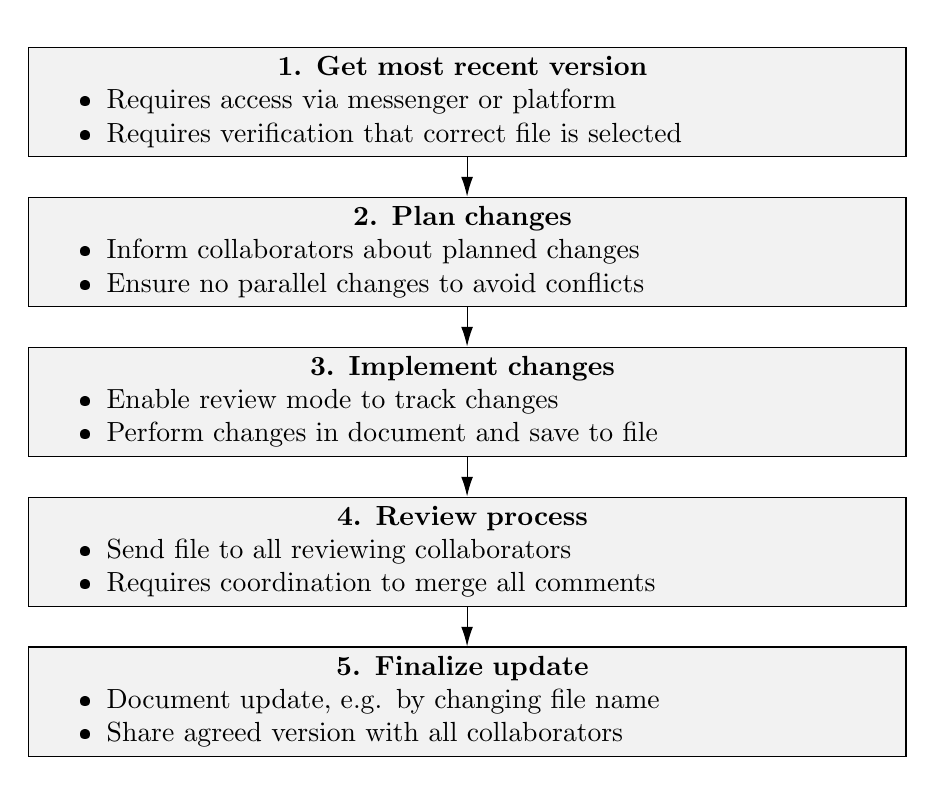
\begin{tikzpicture}

    \tikzset{block/.style= {draw, rectangle, align=center,minimum width=1cm,minimum height=0.5cm}}

    \node[](anchor){};

    \node [block, text width = .9\columnwidth,fill=gray,fill opacity = 0.1, text opacity = 1, below = 0cm of anchor]  (get_recent) {
            \textbf{1. Get most recent version}
            \vspace{-.8em}
            \begin{itemize}
                \setlength\itemsep{-.4em}
                \item Requires access via messenger or platform
                \item Requires verification that correct file is selected
            \end{itemize}};

    \node [block, text width = .9\columnwidth,fill=gray,fill opacity = 0.1, text opacity = 1, below = 0.5cm of get_recent]  (plan_changes) {
            \textbf{2. Plan changes}
            \vspace{-.8em}
            \begin{itemize}
                \setlength\itemsep{-.4em}
                \item Inform collaborators about planned changes
                \item Ensure no parallel changes to avoid conflicts
            \end{itemize}};

    \node [block, text width = .9\columnwidth,fill=gray,fill opacity = 0.1, text opacity = 1, below = 0.5cm of plan_changes]  (implement_changes) {
            \textbf{3. Implement changes}
            \vspace{-.8em}
            \begin{itemize}
                \setlength\itemsep{-.4em}
                \item Enable review mode to track changes
                \item Perform changes in document and save to file
            \end{itemize}};

    \node [block, text width = .9\columnwidth,fill=gray,fill opacity = 0.1, text opacity = 1, below = 0.5cm of implement_changes]  (review) {
            \textbf{4. Review process}
            \vspace{-.8em}
            \begin{itemize}
                \setlength\itemsep{-.4em}
                \item Send file to all reviewing collaborators
                \item Requires coordination to merge all comments
            \end{itemize}};

    \node [block, text width = .9\columnwidth,fill=gray,fill opacity = 0.1, text opacity = 1, below = 0.5cm of review]  (finalize) {
            \textbf{5. Finalize update}
            \vspace{-.8em}
            \begin{itemize}
                \setlength\itemsep{-.4em}
                \item Document update, e.g. by changing file name
                \item Share agreed version with all collaborators
            \end{itemize}};

    \path[draw, -{Latex[length=2.5mm,width=1.5mm]}]
    (get_recent.south) edge (plan_changes.north)
    (plan_changes.south) edge (implement_changes.north)
    (implement_changes.south) edge (review.north)
    (review.south) to (finalize.north);
\end{tikzpicture}
}
    \caption{Overview of the conventional workflow used for applications such as \ac{ISO} standards.}
    \label{fig:workflow_sota}
\end{figure}

"Who would work this way?", the attentive reader might ask.
These processes occur even in highly technical environments with well-educated employees.
There is significant potential for human error in this process, as humans need to undertake laborious tasks that can be automated.
Standardization efforts are a prominent example in which multiple companies with \ac{IP} right concerns collaborate on documents.
Their company policies often prohibit taking the risk of collaborating on shared document platforms with competitors, so the employees resort to the rather inefficient process of exchanging Word files.

\subsubsection{Research}

Researchers have a wide variety of backgrounds and significant liberties in designing their work environment.
Hence, they commonly apply varying techniques for collaborating on documents.
In research, the conventional workflow described in \autoref{sec:standards-workflow} is used as well as shared drives, \wftw, collaboration platforms such as Overleaf~\cite{overleaf_overleaf_2021}, or \magit.
A unified and efficient workflow could improve scientific collaborations and exchange of ideas.

\subsubsection{Software Development}

In professional software development, efficiency of the development process is critical for economic success.
Hence, companies scrutinize their tools and processes and strive for using efficient tools that enable their developers to work efficiently.
Successful companies rely heavily on using version control for their source code documents.
Most companies also use a variant of version control plus a markup language for documentation, such as Google's g3doc~\cite{winters_software_2020}, an internal wiki instance, or Confluence~\cite{atlassian_confluence_2021}.
Once more, this highlights that companies have found the combination of markup plus version control to be the most efficient collaborative documentation approach to date~\cite{winters_software_2020}.
We therefore next introduce an approach for efficient collaboration using a lightweight markup language and version control.

\section{Proposed Process}
\label{sec:process}

In this section, we present the proposed tooling and workflow for efficient collaborative writing.
The proposed documentation workflow is similar to workflows existing for collaboration on source code documents and incorporates many processes described in \autoref{sec:github}.
Each collaborator has a copy of the repository with all relevant documents.
When a collaborator wants to edit the document, a new branch for the changes is created.
Other collaborators can simultaneously work on the documents, as long as they have agreed to work on different sections/topics, for example through issues.
The entire process is summarized in \autoref{fig:workflow_proposed}.

\begin{figure}[ht!]
    \centering
    \resizebox {.8\columnwidth} {!}{\scalefont{0.9}
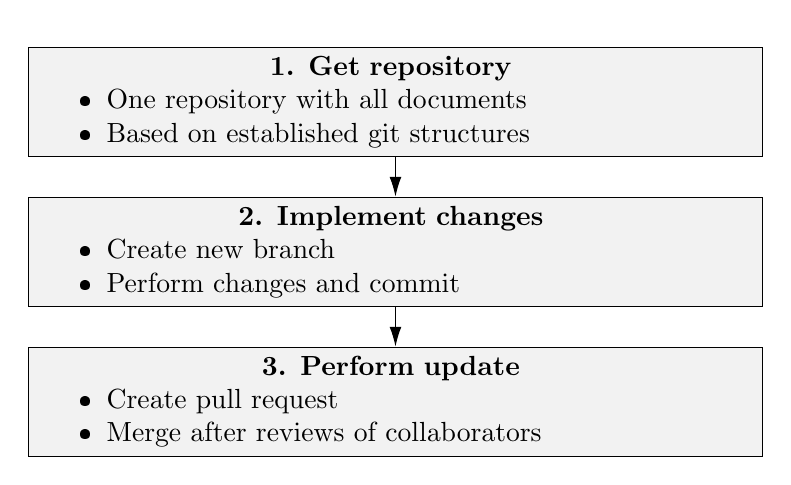
\begin{tikzpicture}

    \tikzset{block/.style= {draw, rectangle, align=center,minimum width=1cm,minimum height=0.5cm}}

    \node[](anchor){};

    \node [block, text width = .75\columnwidth,fill=gray,fill opacity = 0.1, text opacity = 1, below = 0cm of anchor]  (get_repository) {
            \textbf{1. Get repository}
            \vspace{-.8em}
            \begin{itemize}
                \setlength\itemsep{-.4em}
                \item One repository with all documents
                \item Based on established git structures
            \end{itemize}};

    \node [block, text width = .75\columnwidth,fill=gray,fill opacity = 0.1, text opacity = 1, below = 0.5cm of get_repository]  (implement_changes) {
            \textbf{2. Implement changes}
            \vspace{-.8em}
            \begin{itemize}
                \setlength\itemsep{-.4em}
                \item Create new branch
                \item Perform changes and commit
            \end{itemize}};

    \node [block, text width = .75\columnwidth,fill=gray,fill opacity = 0.1, text opacity = 1, below = 0.5cm of implement_changes]  (finalize) {
            \textbf{3. Perform update}
            \vspace{-.8em}
            \begin{itemize}
                \setlength\itemsep{-.4em}
                \item Create pull request
                \item Merge after reviews of collaborators
            \end{itemize}};

    \path[draw, -{Latex[length=2.5mm,width=1.5mm]}]
    (get_repository.south) edge (implement_changes.north)
    (implement_changes.south) to (finalize.north);
\end{tikzpicture}
}
    \caption{Overview of the proposed workflow for efficient large-scale collaborative writing.}
    \label{fig:workflow_proposed}
\end{figure}

While editing, the collaborator creates commits when atomic work-packages are completed.
When the work is done, the author creates a \ac{PR} in the shared repository, other collaborators review, and finally merge the changes.

We select the widely used \git~\cite{chacon_pro_2014} for a prototype of the proposed system.
\git enables the usage of collaboration platforms such as \gh or \gl.
These platforms are rather similar, in particular in terms of collaboration features.
We selected \gh because it has the larger market share of about \SI{88}{\percent}~\cite{gh_market_share_2020}.
The results of \cite{longo_use_2015} and \cite{marquardson_learning_2019} show that the proposed process contains significantly fewer manual, error-prone steps compared to \autoref{fig:workflow_sota}.
Note that the proposed approach is very straightforward since it combines established techniques and well known workflows from software development.
We argue that this is an important quality of the proposed workflow.

To further simplify the usability of the proposed approach, we provide a \gh template repository which allows to use the proposed workflow as a single-click solution.
The template repository can also be used with other platforms such as \gl.
It contains an AsciiDoc template and \ac{CI} configurations running automated checks and validation processes.
This template is publicly available on \gh\footnote{https://github.com/plain-docs/asciidoc-starter}.

\begin{table}[]
\centering
\resizebox{1.0\linewidth}{!}{
\begin{tabular}{l|cccc}
\toprule
&  FID $\downarrow$ & Aesthetic Score~\cite{aesthetic_classifier} $\uparrow$  & CLIP Score~\cite{clip} $\uparrow$ & HPS $\uparrow$  \\
\midrule
SD 1.4     & 19.72 & 5.90 & 0.2816 & 0.1898 \\
Adapted model & 19.35 & 6.06 & 0.2831 & 0.1916 \\
\bottomrule
\end{tabular}
}
\vspace{0.3cm}
\caption{Comparison between the original SD v1.4 and the adapted model.}
\label{tab:comparison}
\end{table}
\section{Conclusion}\label{sec:conclusion}
In this work, we focus on addressing the fundamental challenge of OOD detection tasks, which is how to fully understand the semantic discrepancy between the ID/OOD samples. We reveal that the key to success in the realistic SCOOD task is to allocate as many ID samples in the unlabeled set correctly as possible. To this end, we propose a novel uncertainty-aware optimal transport scheme that introduces class-specific energy scores as guidance for effective label assignment. Experimental results show that our method achieves better performance than previous state-of-the-art methods on SCOOD benchmarks.

\textbf{Limitations.} In addition to temperature scaling, other techniques such as feature clipping applied in ReAct~\cite{sun2021react} also enhance the performance of energy score, so how to obtain an OOD score that best fits the SCOOD task can be further explored. Moreover, a setting highly related to SCOOD has been proposed in \cite{katz2022training} and formulated as a constrained optimization problem. We will also theoretically analyze these practical OOD settings in our feature work.

% \section*{Acknowledgments}
\textbf{Acknowledgments.} 
This work is supported by National Key R\&D Program of China under Grant 2020AAA0105701, National Natural Science Foundation of China (NSFC) under Grants 61872327, Major Special Science and Technology Project of Anhui, National Natural Science Foundation of China (62033012) and Ant Group through Ant Research Intern Program.


%% References
\bibliographystyle{ACM-Reference-Format}
\bibliography{references}

\end{document}
